\documentclass[12pt,a4paper]{article}

\usepackage[utf8]{inputenc}
\usepackage[portuguese]{babel}
\usepackage[T1]{fontenc}
\usepackage[left=2.5cm,right=2.5cm,top=2cm,bottom=2cm]{geometry}
%\usepackage{fancyhdr}
%\pagestyle{fancy}
\usepackage{graphicx}
\usepackage{color}
\usepackage{indentfirst}
\usepackage{wrapfig}
\usepackage{lipsum}
\usepackage{setspace}
\usepackage{adjustbox}


\usepackage{microtype} % Improves typography
\usepackage{gfsdidot} % Use the GFS Didot font: http://www.tug.dk/FontCatalogue/gfsdidot/


% Create a new command for the horizontal rule in the document which allows thickness specification
\makeatletter
\def\vhrulefill#1{\leavevmode\leaders\hrule\@height#1\hfill \kern\z@}
\makeatother
\parindent 1cm

 \renewcommand{\rmdefault}{phv} % Arial
 \renewcommand{\sfdefault}{phv} % Arial

\title{Carta recomendação}
%\author{}

\thispagestyle{empty}

\begin{document}


\begin{wrapfigure}[2]{l}{7cm}

\includegraphics[scale=0.111]{logo-documentos.png}
\end{wrapfigure}



\noindent 
\begin{flushright}
\begin{scriptsize}
Francisco Rouxinol \\
Instituto de Física Gleb Watghin\\
Rua Sergio Buarque de Holanda, 777\\
13083-859, Campinas, SP \\
e-mail: rouxinol@unicamp.br\\
tel: +55(19)3521-5462\\
% \hspace{-0.5cm} 
\vhrulefill{1pt} \\ % 
\end{scriptsize}
\end{flushright}

% \singlespacing %Para um espaçamento simples
% \onehalfspacing %Para um espaçamento de 1,5
%\doublespacing %Para um espaçamento duplo 

% $ $\\


% \singlespacing %Para um espaçamento simples
% \large 
\begin{flushleft}
\textbf{Projeto Principal}: “Algoritmo quântico de procura de Grove: implementação da simulação em computadores clássicos e quânticos”\\
\textbf{Grande Área de conhecimento:} Ciências Exatas e da Terra\\
\textbf{Grande Área de conhecimento: }Ciências Exatas e da Terra\\
\textbf{Área de Conhecimento:} Física\\
\textbf{Subárea de Conhecimento: }Física da Matéria Condensada\\
\textbf{Aluno(a):} Daniel Benvenutti\\
\textbf{Orientador: }Francisco Rouxinol\\
\textbf{Instituição:} Instituto de Física Gleb Wataghin, UNICAMP\\
\textbf{Palavras chaves:} Eletrodinâmica Quântica, Computação Quântica e Informação\\
\textbf{Referente:} Primeiro Relatório
\end{flushleft}


%  \singlespacing %Para um espaçamento simples
\subsection{Registrador Quântico}
A primeira parte do projeto e construir o simulador. Para simular o estado de $N$ qubits precisamos de um vetor de  $2^{N}$ elementos.
por exemplo um vetor de 3 qubits com 8 elementos.


\emph{ Psi=[0,\, 0,\, 0,\, 0,\, 0,\, 0,\, 0,\, 0]}

Em seguida precisamos poder medir esse estado quântico. Uma medida é representada por por uma escolha aleatória do computador levando como pesos probabilísticos os elementos do vetor de estado com maior módulo complexo ao quadrado.

\emph{[0,\, 1,\, 0,\, 0,\, 0,\, 0,\, 0,\, 0]}

Por exemplo tem 100\% de chance de ser medida como o segundo elemento

\emph{[0.5,\, 0.5,\, 0.5,\, 0.5,\, 0,\, 0,\, 0,\, 0]}

Tem $|0.5|^{2}=1/4$ de chance de ser medido no primeiro, segundo, terceiro ou quarto estados.

Cada estado nesse vetor representa uma compibanção das medidas possíveis dos qubits. O primeiro estado é $|000\rangle$ o segundo é $|001\rangle$, o terceiro é $|010\rangle$ e assim por diante até o oitavo.
\subsection{Portas quânticas}
Agora vamos as portas. A primeira porta é a porta de Hadamard. Um dos efeitos interessantes dela é que ela coloca um qubit em uma superposição de dois estados. 
por exemplo, o código:
\begin{verbatim}
    
qubit=[1,0]
qubit=hadamard(qubit, 1, 1) # hadamard no primeiro qubit
print(qubit)

\end{verbatim}

retorna

[0.707106781186547, 0.707106781186547]

Temos também a porta de mudança de fase. Ela muda a fase complexa do elemento do vetor que descreve o qubit que é $|1\rangle$.
Então se usarmos uma dessas portas:

\begin{verbatim}
    qubit=[0,1]
qubit=muda_fase(qubit, 1, math.pi/2, 1)
print(qubit)
medir_n(qubit, 100, 1)
\end{verbatim}

obteremos:

[0, 0 + 1.0*I]

Que tem um número imaginário puro no segundo elemento do vetor já que ele é $|1\rangle$ no caso de um único qubit e que a fase da nossa mudança é $\pi/2$.


 Portões CNOT são portas quânticas NOT (ou NÃO) controladas e funcionam da seguinte maneira: Há um qubit controlador e um qubit que sofre a operação NOT. Se e somente se o qubit controlador é $|1\rangle$ que o outro qubit é invertido de $|1\rangle$ para $|0\rangle$ ou de $|0\rangle$ para $|1\rangle$. Se o controlador for $|0\rangle$ o controlado mantém o seu estado. O qubit controlador não é alterado. Com essa porta podemos fazer o estado de emaranhamento quântico:
 
 \begin{verbatim}
     Psi=[0]*8
seta_base(Psi,0)

#hadamard no segundo qubit para coloca-lo numa superposição
Psi=hadamard(Psi, 2, 3)  
#CNOT para emaranhar os qubits
Psi=cnot3(Psi, 3)

print(Psi)
medir_n(Psi, 1000, 3)
 \end{verbatim}

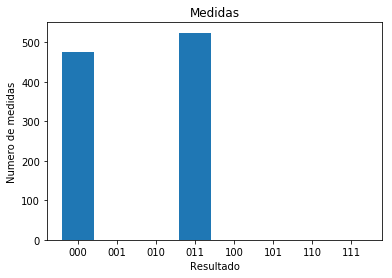
\includegraphics[]{relatorio-superposicao.png}


Obteremos uma superposição entre os dois estados $|000\rangle$ e $|011\rangle$ logo há uma correlação na medida do segundo e terceiro qubit. Se um é medido zero o outro também e o mesmo com 1.

[0.71, 0, 0, 0.71, 0, 0, 0, 0]
\subsection{Algoritmo de Groover}
O algoritmo de Groover é um algoritmo de busca. Dado um vetor de de possíveis resṕostas com uma delas certa ele indica qual é a correta. Com uma algoritmo normal de varredura em um computador clássico no pior caso temos que verificar todos os $n$ elementos. Já no algoritmo de Groover precisamos de apenas $\sqrt{n}$ buscas.

Apesar disso a nossa lista precisa ser armazenada num oráculo quântico que é um operador que será utilizado nos nossos qubits. O que é mais dificil.


O algoritmo de Groover funciona usando uma técnica chamada amplificação de amplitude. Onde a fase do elemento do vetor que é a resposta é invertida e em seguida com o operador de difusão de Groover é amplificada. Isso é repetido um número ótimo de vezes que deixa a resposta correta com uma maior probabilidade de ser medida.

Aqui temos uma exeução do código:
\begin{verbatim}
    Psi=[1,0,0,0,0,0,0,0]

count=1
while count <= 3:    #passa o loop pelo vetor psi
    Psi=hadamard(Psi, count, 3) #hadamard em todos os qubits
    count = count + 1

resposta=6

#blocos do operador de difusao de groover
Psi=bloco_groover(Psi, 3, resposta)
Psi=bloco_groover(Psi, 3, resposta)

print(Psi)
medir_n(Psi, 1000, 3)
\end{verbatim}

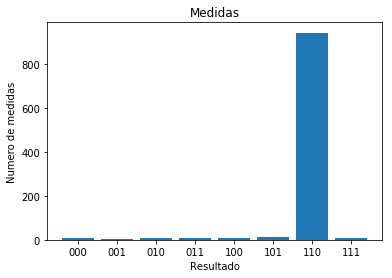
\includegraphics[]{relatorio_groover.png}


O vetor resposta encontrado é:


[-0.08, -0.08, -0.08, -0.08, -0.08, -0.08, 0.97, -0.08]

Onde a amplitude do 7 elemento '110' (6  já que se começa do 0) é $0.97$ enquanto a dos outros é de apenas $-0.08$.


Em seguida avaliamos o desempenho da simulação do algoritmo de Groover no meu computador. Abaixo os resultados:

\begin{table}[htb]

\begin{adjustbox}{center}
\begin{tabular}{|l|l|}  
\hline
Qubits  & tempo \\ \hline
1  & 1.20s \\ \hline
2  &  1.15s\\ \hline
3  &   1.36s\\ \hline
4  &  3.51s\\ \hline
5  &  29.33s\\ \hline
6  &   353.69s\\ \hline

\end{tabular}
\end{adjustbox}
\end{table}


Depois o algoritmo de Groover foi executado utilizando-se matrizes exparsas. Que são muito úteis nessas simulações já que as matrizes dos operadores tem muitos zeros.

\begin{verbatim}
    
qubits=input()
resposta=1

Psi=[0]*2**qubits
Psi[0]=1

count=1
while count <= qubits:    #passa o loop pelo vetor psi
        Psi=sp_hadamard(Psi, count, qubits) #hadamard em todos os qubits
        count = count + 1

#blocos do operador de difusao de groover
count=1
   #passa o loop pelo vetor psi
while count <= round(math.pi/4*math.sqrt(2**qubits)): 
        Psi=sp_bloco_groover(Psi, qubits, resposta)
        count = count + 1
print(Psi)
print("done")

\end{verbatim}


\begin{table}[htb]
\centering
\begin{adjustbox}{center}
\begin{tabular}{|l|l|}  
\hline
Qubits  & tempo \\ \hline
1  & 0.86s \\ \hline
2  &  0.92s\\ \hline
3  &   0.91s\\ \hline
4  &  0.97s\\ \hline
5  &  1.04s\\ \hline
6  &   1.16s\\ \hline

7  &   1.42s\\ \hline

8  &   2.16s\\ \hline

9  &   5.06s\\ \hline

10  &   19.40s\\ \hline

11 &   105.38s\\ \hline

12 &   626.17s\\ \hline

13 &   353.69s\\ \hline

\end{tabular}
\end{adjustbox}
\end{table}
Nota-se a grande melhoria no desempenho e como é possível utilizar um número muito maior de qubits com o mesmo computador.

\subsection{Algoritmo de Shor}
 O algoritmo de Shor é um algoritmo de fatoração de números inteiros. Um dos seus passos é acelerado se executado em um computador quântico. Abaixo os passos do algoritmo:

Dado um número $C$ que se deseja encontrar os fatores:

\begin{enumerate}

 \item Cheque se $C$ é impar e não é potência de algum inteiro pequeno. Se for um desses encontramos um fator de $C$ e terminamos.

 \item Pegue qualquer inteiro no intervalo $1 < a < C$.

 \item Encontre o $mdc(a, C)$ (maior divisor comum). Se o mdc for maior que 1 por sorte, encotramos ja um fator de C e terminamos.

 \item Encontre o menor inteiro $p$ tal que $a^{p} \equiv 1\, mod\, C$. A expressão  $p \equiv q \, mod\, C$ quer dizer a congruência modular. Ou seja $p-q$ é um inteiro multiplo de C. Isso pode ser escrito também como $p\, mod\, C = q\, mod\, C$.

 \item Se $p$ é impar ou se $p$ é par e $a^{p/2} \equiv -1\, mod\, C$ volte para 2 e escolha um novo $a$.

 \item Os números $P_{\pm} = mdc( a^{p/2} \pm 1, C)$ são fatores não triviais de C.

\end{enumerate}

O computador quântico é responsável pelo 4º passo desse algoritmo. O resto dos passos como encontrar o mdc são feitos rapidamente em um computador clássico.

Esse passo se chama encontrar o período pois $f(x)=a^{x} \, mod \, C$ é uma função periódica com período $p$. Dividimos o registrador quântico em duas partes: o registrador $x$ com $L$ qubits iniciado em $|0...0\rangle$ e o $f$ com $M$ qubits iniciado em $|0...01\rangle$:

O quarto passo:


\begin{enumerate}
\item Aplique portas de Hadamard em todos os L qubits do registrador $x$, representado por $H^{\otimes L}$. Isso coloca o registrador $x$ numa superposição de todos os $2^{L}$ estados possíveis

\item Multiplique o registrador $f$ por $a^{x} \, mod \, C$ fazendo com que fique com o valor de $f(x)$.

\item Meça o registrador $f$ (esse passo é opcional)

\item Faça uma transformada de fourier quântica inversa (IQFT em inglês) no registrador $x$. A IQFT permite encontrar o período da função.

\item Meça a saída $\bar{x}$ de do IQFT (lembrando que temos que ler a saída do IQFT na direção contrária).  Shor provou que $\bar{x}/2^{L}$ é igual a aproximadamente $s/p$ onde $s$ é um inteiro qualquer. Usamos isso para encontrar $p$. Por exemplo $\bar{x}/2^{L} = 0.32 \cong 1/3 = 2/6 = 3/9$ então $p$ é $3, 6, 9, \cdots$ Checamos em seguida esses valores para ver se $a^{p} \equiv 1\, mod\, C$.

\end{enumerate}


\begin{verbatim}
a=2

#psi comeca em |0000001>
qubits=7
psi=[0]*(2**qubits)
seta_base(psi,1)


#coloca em superposicao os bits de L
psi=sp_hadamard(psi, 3, qubits) #hadamard em l0 
psi=sp_hadamard(psi, 2, qubits) #hadamard em l1 
psi=sp_hadamard(psi, 1, qubits) #hadamard em l2 
print "qubits L em superposição"
print psi

#parte de f de x
#multiplica por a se l0=1
psi=shor_fx(psi, 1, a, 15, 3, 4) 
 #multiplica por a^2 se l1=1
psi=shor_fx(psi, 2, a**2, 15, 3, 4)
#multiplica por a^3  se l2=1
psi=shor_fx(psi, 3, a**4, 15, 3, 4) 
# terminado e multiplicando por a^(l2l1l0)

print "-------------------------"
print "matrizes de permutação aplicadas para econtrar f(x)"
print psi

#IQFT transformada de fourier quantica inversa
psi=sp_hadamard(psi, 1, qubits) #hadamard em l2

#mudanca de fase de pi/2 controlada por l2 em l1
psi=sp_Cfase(psi, 2, 1, qubits, math.pi/2) 

#mudanca de fase de pi/4 controlada por l2 em l0
psi=sp_Cfase(psi, 3, 1, qubits, math.pi/4) 

psi=sp_hadamard(psi, 2, qubits) #hadamard em l1

#mudanca de fase de pi/2 controlada por l2 em l1
psi=sp_Cfase(psi, 3, 2, qubits, math.pi/2) 

psi=sp_hadamard(psi, 3, qubits) #hadamard em l0 

print "-------------------------"
print "transformada de fourier quântica inversa aplicada para encontrar o período da função"
print psi

medir_xbarra_shor(Psi, 1000, 3, 4)
\end{verbatim}

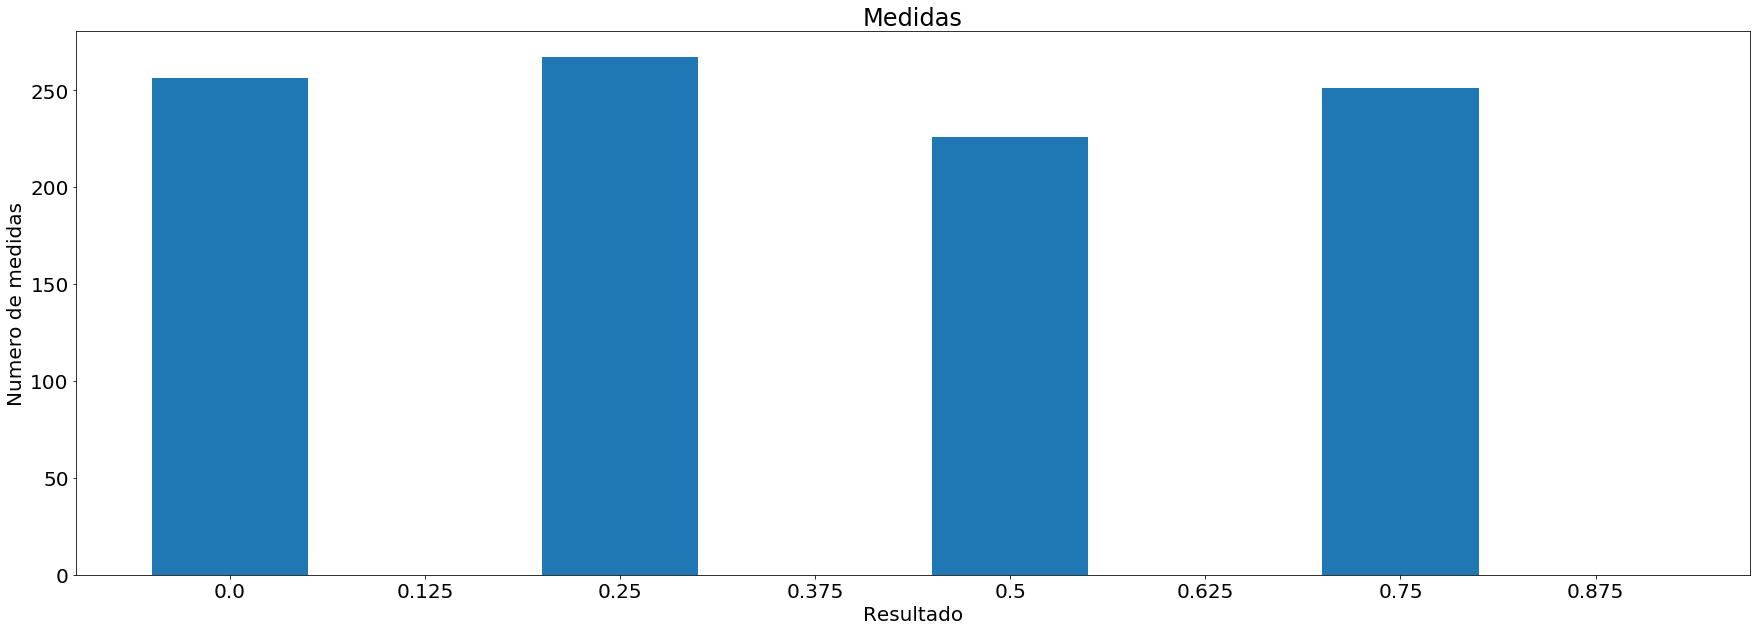
\includegraphics[scale=0.25]{relatorio-shor1.png}

Agora medimos o resultado no registrador obtendo varios valores para $\bar{x}/2^{L}$ onde $\bar{x}$ é o valor do registrador $x$ após a aplicação do IQFT com os bits invertidos. Esses valores são a frequência da função e seus harmônicos $s\omega$ onde $s$ é um inteiro. Ou seja obtemos como medida um valor $s/p$ para a medida de $\bar{x}/2^{L}$ onde $s$ é um inteiro qualquer e $p$ é o valor procurado do período para o algoritmo de Shor. Como obtemos quatro valores principais podemos concluir que p=4. Na prática, podemos contar o número de picos principais na medidas de saída. 4 picos equivale a um periodo de 4 por exemplo. Também podemos usar frações parciais para aproximar o valor desejado a partir das resultados da saída do computador quântico.


Também foi feito uma simulação do Shor para um número N arbitrário de qubits:

\begin{verbatim}
    a=10

L=6
M=6
C=21

#psi comeca em |00 ... 01>
qubits=L+M
psi=[0]*(2**qubits)
seta_base(psi,1)


#coloca em superposicao os bits de L
j=1
while j<=L :
    psi=sp_hadamard(psi, j, qubits) #hadamard
    print "had", j
    j = j + 1
    

#parte de f de x
j=1
while j<=L :
#multiplica por a^3  se l2=1 terminado e multiplicando por a^(l2l1l0)
    psi=shor_fx(psi, j, a**(2**(j-1)), C, L, M) 
    print "fx", j
    j = j + 1
    

#IQFT transformada de fourier quantica inversa
i=1

while i <= L:
    
    psi=sp_hadamard(psi, i, qubits) #hadamard em l2 
    #print "hadamard", i
    j=1
    while j <= L-i:
     #mudanca de fase de pi/2 controlada por l2 em l1
        psi=sp_Cfase(psi, i+j, i, qubits, math.pi/(2**j))
        #print i+j, "controls pi/",2**j, "on", i
        j = j + 1
    print "IQFT", i
    i = i + 1
    

print 'terminado'

#plota
Psi=psi.toarray()[0]
medir_xbarra_shor(Psi, 1000, L, M)

\end{verbatim}
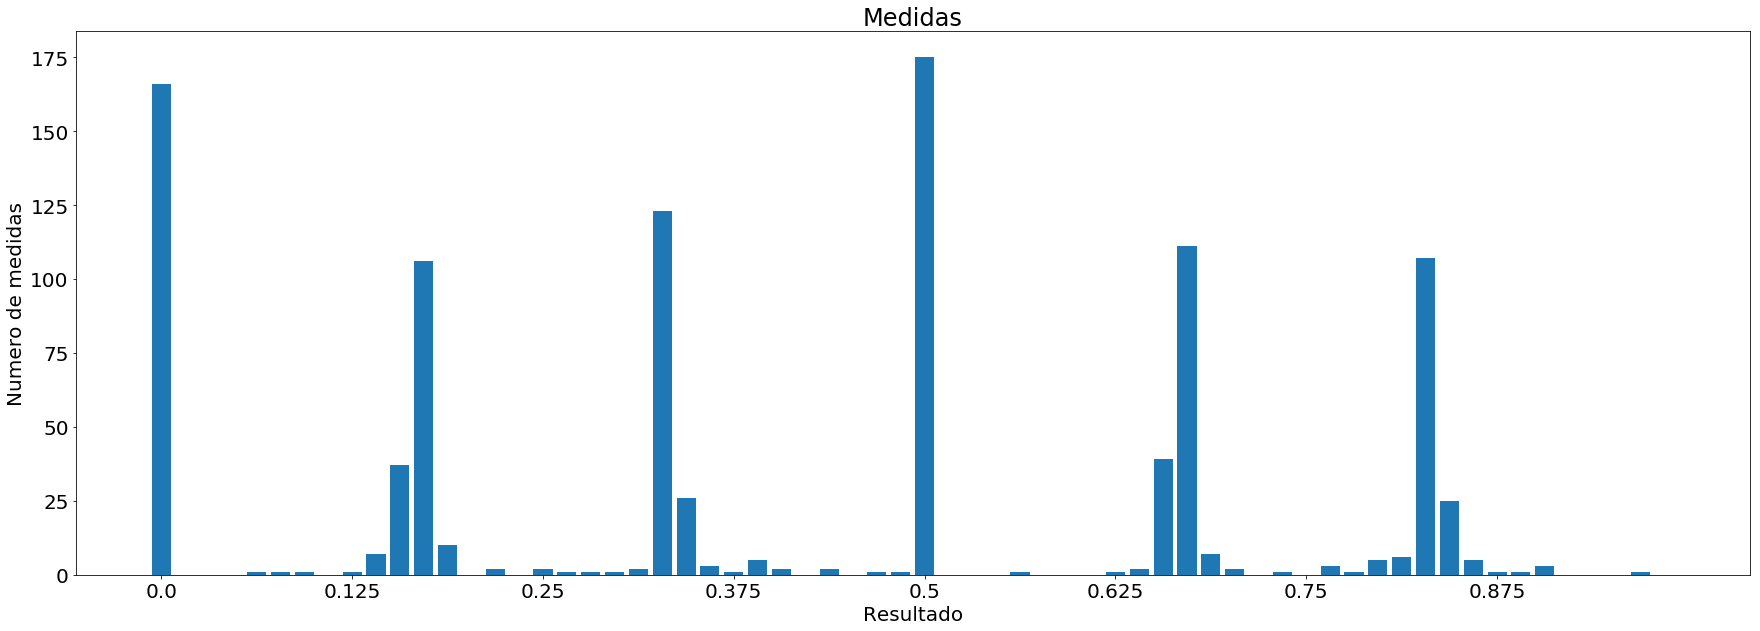
\includegraphics[scale=0.3]{relatorio-shor2.png}


\end{document}

